
% 122

\subsubsection{Conclusion et inteprétation physique}% d
Nous venons donc de montrer que le paquet d'ondes $|\ \psi^+\mt{(t)}>$,
formé à l'aide des états stationnaires de collision, se trouve dans le
passé \ul{lointain} (en fait si t << $-\hbar/\Delta\mt{E}$) pratiquement confondu avec le
paquet d'ondes libres $|\ \phi\mt{(t)}>$ construit à l'aide des \ul{mêmes} coefficients.

De même le paquet d'ondes $|\ \psi^-\mt{(t)}>$, dans le \ul{futur lointain}
(en fait si t >> $\hbar/\Delta\mt{E}$) sera pratiquement confondu avec le paquet d'ondes
libres $|\ \phi\mt{(t)}>$ correspondant,

De tels résultats sont extrêmement importants en ce qui concerne
la théorie des collisions : dans une expérience de collision, on prépare
en effet les particules incidentes, dans un passé lointain, loin de la
cible, dans une région où le potentiel V n'existe pas.

L'état initial correspond donc à un paquet d'ondes libres
$|\ \phi\mt{(t)}>$ constitué à l'aide des $|\ \phi_\mt{i}>$. Mais les $|\ \phi_\mt{i}>$ n'étant pas des
états propres de H, l'évolution d'un tel paquet d'ondes pendant et après
la collision n'est pas facile à calculer. L'intérêt des états stationnaires de
collision apparaît ici : nous venons en effet de montrer que dans
le passé lointain (c'est-à-dire longtemps avant la collision), il revient
au même de développer le paquet d'ondes suivant les états libres $|\ \phi_\mt{i}>$ ou
les états stationnaires de collision $|\ \psi_\mt{i}^+>$. On peut donc prendre pour
état initial de la collision un état $|\ \psi^+\mt{(t)}>$, au lieu de $|\ \phi\mt{(t)}>$ Les
$|\ \psi_\mt{i}^+>$ étant, eux, des états propres de H, l'évolution de $|\ \psi^+\mt{(t)}>$ est
connue et conduit pour le futur lointain (c'est-à-dire longtemps après la
collision) à la formule (47-b). Cette formule, qui décrit donc l'état,
après collision d'un paquet d'ondes libres incident, est très importante
car c'est elle qui va nous permettre de calculer les sections efficaces
de collision.

Nous pouvons déjà, à ce stade, remarquer qu'elle représente le
paquet d'ondes libres incident auquel s'ajoute un paquet d'ondes libres,
diffusé dans toutes les directions de l'espace, mais dont le module du
vecteur d'onde est centré autour de la valeur $\overline{\mt{k}_\mt{i}}$ du paquet incident
% 123
(en raison du terme $\mt{C}(\mt{k}_\mt{j }\Omega_\mt{i})$ de la relation (47-c) ce qui n'est autre
que l'expression de la conservation de l'énergie au cours de la collision élastique.

Enfin, si on veut avoir une représentation spatio-temporelle
de la collision, il faut passer en représentation r et appliquer la méthode de la
phase stationnaire pour déterminer la répartition à chaque
instant du paquet d'ondes. On obtient alors l'image représentée par les
figures suivantes (cf Messiah, p. 316 et suivantes).\begin{center}
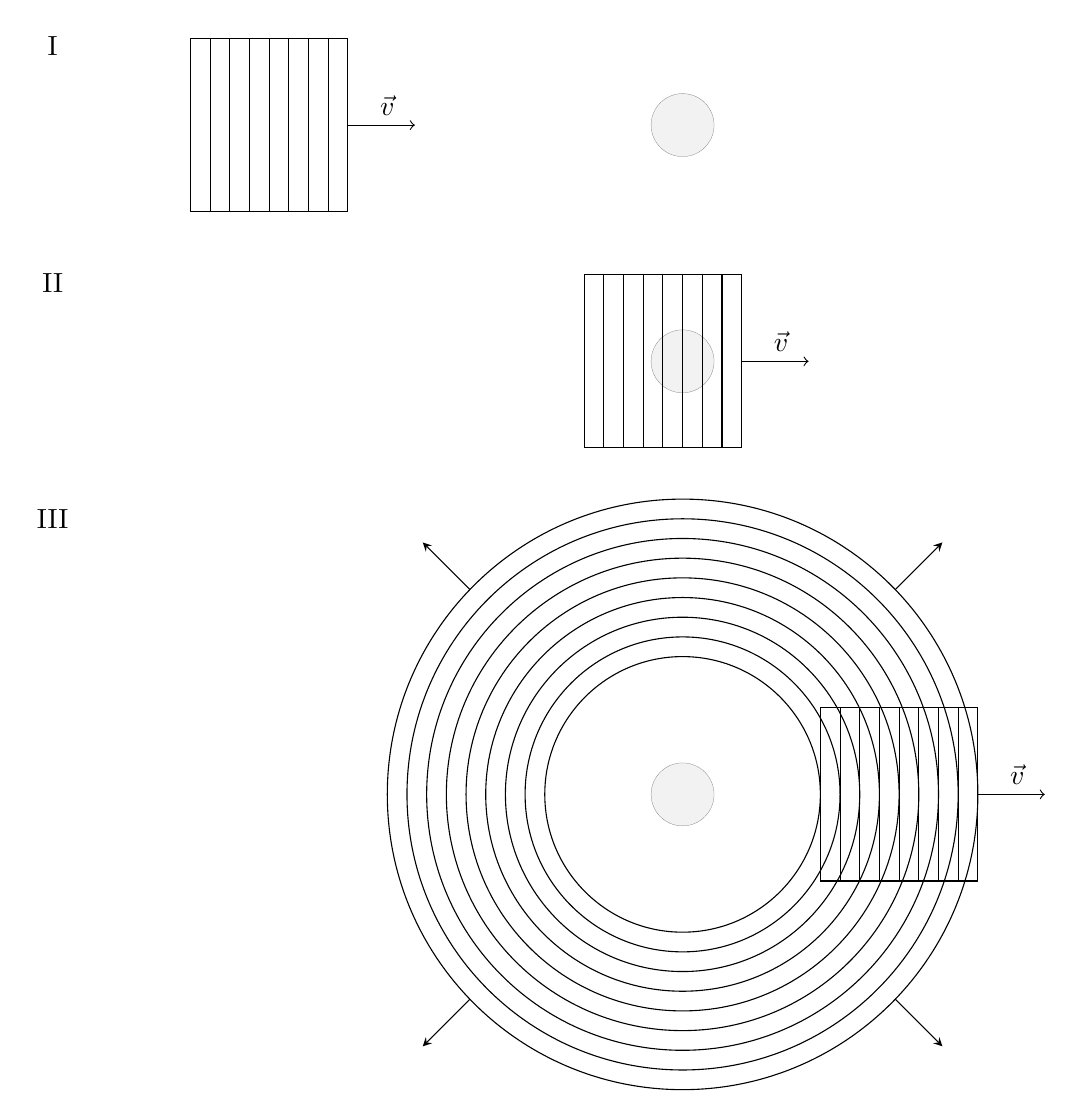
\begin{tikzpicture}
  \def\lond{0.25}
  %Potentiel I
  \fill[color=gray!10,draw=gray, ultra thin] (0,3) circle (0.4);
  \draw (-8,4) node {I};
\begin{scope}[xshift=-5 cm,yshift=3 cm]
  %Onde I
  \foreach \s in {-5,-4,...,3}
    {\draw (\s*\lond,-1.1) -- (\s*\lond,1.1);}
  \draw [->] (0.75,0) -- (1.6,0);\draw (1.25,0) node [above]{$\vec{\mt{v}}$};
  \draw (0.75,1.1) -- (-1.25,1.1); \draw (0.75,-1.1) -- (-1.25,-1.1);
\end{scope}
  %Potentiel II
  \draw (-8,1) node {II};
  \fill[color=gray!10,draw=gray, ultra thin] (0,0) circle (0.4);
  %Onde II
  \foreach \s in {-5,-4,...,3}
    {\draw (\s*\lond,-1.1) -- (\s*\lond,1.1);}
  \draw [->] (0.75,0) -- (1.6,0);\draw (1.25,0) node [above]{$\vec{\mt{v}}$};
  \draw (0.75,1.1) -- (-1.25,1.1); \draw (0.75,-1.1) -- (-1.25,-1.1);
  %Potentiel III
  \draw (-8,-2) node {III};
  \fill[color=gray!10,draw=gray, ultra thin] (0,-5.5) circle (0.4);
\begin{scope}[xshift=3 cm,yshift=-5.5 cm]
  %Onde III
  \foreach \s in {-5,-4,...,3}
    {\draw (\s*\lond,-1.1) -- (\s*\lond,1.1);
    \draw (-3,0) circle(3+\s*\lond);}
  \draw [->] (0.75,0) -- (1.6,0);\draw (1.25,0) node [above]{$\vec{\mt{v}}$};
  \draw (0.75,1.1) -- (-1.25,1.1); \draw (0.75,-1.1) -- (-1.25,-1.1);
  \draw [>=stealth,->] (-0.3,2.6) -- (0.3,3.2);\draw [>=stealth,->] (-5.7,2.6) -- (-6.3,3.2);
  \draw [>=stealth,->] (-0.3,-2.6) -- (0.3,-3.2);\draw [>=stealth,->] (-5.7,-2.6) -- (-6.3,-3.2);
\end{scope}
\end{tikzpicture} \end{center}
% 12

Nous avons ainsi établi un nouveau lien physique entre les
états stationnaires de collision $|\ \psi^+_\mt{i}>$ et les états libres $|\ \phi_\mt{i}>$, par
l'intermédiaire des paquets d'ondes. C'est cette dernière propriété des
$|\ \psi^+_\mt{i}>$ qui est le plus de signification physique car nous venons de montrer
qu'elle est liée de façon évidente à la description même de l'expérience
physique. Elle va nous permettre également d'éclairer sous un jour nouveau
"l'approche adiabatique" ou celle de l'introduction progressive de l'état
"initial" faites aux \S 1 et 2 :

\subsubsection{Lien avec les 2 autres approches physiques (\S 3.1 et 3.2)} % e) 
Plus la fonction de répartition C($\mt{k}_\mt{i},\Omega_\mt{i}$) est étroite autour
des valeurs moyennes $\overline{\mt{k}_\mt{i}}$ et $\overline{\Omega_\mt{i}}$,
plus le paquet d'ondes $|\ \phi(0)>$ est proche
de l'état stationnaire $|\ \overline{\phi_\mt{i}}>$ et plus le paquet d'ondes $|\ \psi^+(0)>$ est proche
de l'état stationnaire de diffusion $|\ \overline{\psi^+_\mt{i}}>$, $|\ \phi_\mt{i}>$
et $|\ \psi_\mt{i}^+>$ sont les
paquets d'ondes à l'instant t = 0 à la limite où on a remplacé C($\mt{k}_\mt{i},\Omega_\mt{i}$)
par une fonction de Dirac au point $\overline{\mt{k}_\mt{i}},\overline{\Omega_\mt{i}}$.
Mais tant que C($\mt{k}_\mt{i},\Omega_\mt{i}$) possède
une certaine dispersion \ul{$\Delta$E en énergie}, on a vu qu'il existe un temps
t<<$-\frac{\hbar}{\Delta\mt{E}}$, tel que le "paquet de collision" qui est très proche de l'état
stationnaire de collision à l'instant t = 0, se réduise à ce temps au "paquet libre",
qui est lui très proche de l'état libre $|\ \phi_\mt{i}>$.

Dans les deux autres approches physiques que nous avons données,
le fait d'établir la perturbation sur un intervalle de temps $\hbar/\epsilon$ ou d'introduire
progressivement l'état initial sur un intervalle de temps $\hbar/\epsilon$
fait que l'état obtenu à l'instant t = 0 n'est pas (pour $\epsilon\neq0$) un état
propre de H, Il existe sur son énergie une incertitude, qui provient de sa
préparation même de l'ordre de $\epsilon$. On peut encore dire, qu'avant de faire
tendre $\epsilon\to0$, l'état obtenu à l'instant t $=$ 0, $|\ \psi^+_\mt{i}>_\epsilon$ qui obéit à l'équation (35 après intégration).
\[
|\;\psi_\mt{i}^+(0)>_\epsilon\,=|\;\phi_\mt{i}>+\frac{1}{\mt{E}_\mt{i}-\mt{H}\pm\mt{i}\epsilon}\mt{ V }|\;\phi_\mt{i}>
\]
% 125
est une superposition d'états stationnaires $|\ \psi^+_\mt{i}>$ avec une dispersion
de l'ordre de $\epsilon$. $|\ \psi^+_\mt{i}>_\epsilon$ représente donc en quelque sorte un "paquet
d'ondes" de largeur en énergie $\epsilon$, auquel nous pouvons appliquer les résultats précédents.

\vspace{1.5cm}
En d'autres termes, le fait d'introduire progressivement la
perturbation (ou l'état initial) sur un temps de l'ordre de $\hbar/\epsilon$ est une
façon commode de simuler un paquet d'ondes de dispersion en énergie $\epsilon$ {\footnotesize (On peut encore dire qu'il revient au même de "faire passer" le paquet
d'ondes pendant un temps $\hbar/\Delta\mt{E}$ devant la perturbation (ce qui correspond
à l'expérience \ul{physique réelle}) ou, par exemple, de brancher la perturbation sur
une onde plane libre pendant le même temps (\S 3-1).)}
Il est de plus beaucoup plus aisé de travailler avec des états du type
$|\ \psi^+_\mt{i}>_\epsilon$ qu'avec des paquets d'ondes. C'est 1à tout l'intérêt de la
\ul{théorie formelle des collisions} qui est basée sur l'emploi systématique
des états $|\ \psi^+_\mt{i}>_\epsilon$.

Il faut cependant prendre une \ul{précaution essentielle} : le
paramètre $\epsilon$, qui a été introduit dans tous les calculs a, ainsi que nous
venons de le voir, une signification physique très \ul{simple et fondamentale} :
il représente l'incertitude sur l'énergie dans l'expérience \ul{physique réelle} :
cette incertitude existe toujours. Tous les calculs mathématiques conduisent
aux grandeurs \ul{physiques} devront donc être faits avec un $\epsilon$ \ul{fini différent de
zéro}. Ce n'est qu'à la fin des calculs qu'on pourra faire tendre $\epsilon$ vers zéro.
Deux cas peuvent alors se présenter : ou bien la limite existe et elle
représente la grandeur physique cherchée dans le cas où la définition en
% 126
énergie de l'expérience était très bonne; ou bien la limite n'existe pas
ou est absurde : cela signifie alors que le résultat physique dépend crucialement
de la forme du paquet d'ondes et la théorie formelle des collisions
ne peut s'appliquer : il faut raisonner sur les paquets d'ondes.
En d'autres termes, tant que le résultat physique est indépendant de la
forme du paquet d'ondes incident, la théorie formelle des collisions
s'applique et permet de résoudre les problèmes de façon élégante. Nous
allons d'ailleurs en voir un exemple en appliquant toute l'étude précédente à la
théorie des collisions.

\section{Application de l'étude précédente : Théorie des collisions}% D
\subsection{Définition de la section efficace différentielle de diffusion}% 1 

\subsubsection{Probabilité de transition}% a

Soit P($\Omega_\mt{j}$, t) d$\Omega_\mt{j}$ la probabilité de trouver à l'instant t le
vecteur d'onde de 1a particule dans l'angle solide ($\Omega_\mt{j}$, $\Omega_\mt{j}+$d$\Omega_\mt{j}$).

Soit W($\Omega_\mt{j}$, t) la dérivée $\frac{\mt{d}}{\mt{dt}}$ P($\Omega_\mt{j}$, t).

La quantité d$\Omega_\mt{j}$ dt W($\Omega_\mt{j}$) représente la probabilité pour
qu'entre les instants t et t $+$ dt la particule ait été diffusée dans
l'angle solide ($\Omega_\mt{j}$, $\Omega_\mt{j}+$d$\Omega_\mt{j}$).

Si W($\Omega_\mt{j}$, t) est indépendent du temps, on définit alors W($\Omega_\mt{j}$)
comme la \ul{probabilité de} \ul{transition par unité de temps}.

Enfin, si $\vec{\mt{k}}_\mt{j}\neq\vec{\mt{k}}_\mt{i}$ vecteur d'onde de la particule incidente, il
est évident que P($\Omega_\mt{j},-\infty)=0$.

P($\Omega_\mt{j},+\infty)$ d$\Omega_\mt{j}$ représente la probabilité totale pour qu'après
la collision da particule ait été diffusée dans l'angle solide
($\Omega_\mt{j}$, $\Omega_\mt{j}+$d$\Omega_\mt{j}$) et on a la relation
\[
\mt{P}(\Omega_\mt{j},+\infty)=\int_{-\infty}^{+\infty}\mt{W}(\Omega_\mt{j},\mt{t})\mt{ dt}
\]
% 127
\subsubsection{Flux des particules libres}% b
Supposons maintenant que V = 0 et que la particule est
\ul{toujours libre}.

Appelons $\vec{\mt{J}}(\vec{\mt{r}},\mt{t})$ le flux à l'instant t, au point $\vec{\mt{r}}$ de la
\ul{particule libre} et prenons le point $\vec{\mt{r}}$ à l'intérieur de la zone, d'extension r$_0$
où règne le potentiel V. Le flux $\vec{\mt{J}}(\vec{\mt{r}},\mt{t})$ ne varie d'ailleurs pas
d'un point à l'autre de cette zone si, comme nous en avons fait l'hypothèse,
la largeur du paquet d'ondes est grande devant v.

Soit $\rho(\vec{\mt{r}},\mt{t})$ la densité de probabilité de présence de la
particule libre en $\vec{\mt{r}}$ à l'instant t. On a alors
\[
\vec{\mt{J}}(\vec{\mt{r}},\mt{t})=\rho(\vec{\mt{r}},\mt{t})\;\vec{\mt{v}}=
\rho(\vec{\mt{r}},\mt{t})\;\frac{\hbar\;\overline{\vec{\mt{k}}_\mt{i}}}{\mt{m}}
\]
Soit $\sigma$ une surface située en $\vec{\mt{r}}$ et perpendiculaire à la vitesse initiale
de la particule libre : la probabilité totale pour que la particule
\ul{libre} soit passée à travers $\sigma$ est
\[
\sigma\int_{-\infty}^{+\infty}\mt{J}(\vec{\mt{r}},\mt{t})\mt{ dt}
\]

\subsubsection{Définition de la section efficace différentielle de diffusion}% c

La section efficace différentielle de diffusion pour
l'angle solide $\Omega_\mt{j}$ est une surface $\sigma(\Omega_\mt{j})$ définie de la façon suivante :

La probabilité globale pour que, sous l'effet de V, la particule soit diffusée
dans l'angle solide ($\Omega_\mt{j}$, $\Omega_\mt{j}+$d$\Omega_\mt{j}$) est égale à d$\Omega_\mt{j}$ fois
la probabilité globale pour que la particule passe à travers la surface $\sigma(\Omega_\mt{j})$
si elle restait toujours libre. ($\sigma(\Omega_\mt{j})$ est perpendiculaire à la
vitesse de la particule incidente et située en un point $\vec{\mt{r}}$ où règne le
potentiel V).
% 128
Par définition, on a donc
\[
\sigma(\Omega_\mt{j})\mt{ d}\Omega_\mt{j}\int_{-\infty}^{+\infty}\mt{J}(\vec{\mt{r}},\mt{t})\mt{ dt}
=\mt{ d}\Omega_\mt{j}\mt{ P}(\Omega_\mt{j},+\infty)
\]
Soit
\[
\tag{49}\sigma(\Omega_\mt{j})=\frac{\mt{P}(\Omega_\mt{j},+\infty)}{\int_{-\infty}^{+\infty}\mt{J}(\vec{\mt{r}},\mt{t})\mt{ dt}}
=\frac{\int_{-\infty}^{+\infty}\mt{W}(\Omega_\mt{j},\mt{t})}{\int_{-\infty}^{+\infty}\mt{J}(\vec{\mt{r}},\mt{t})\mt{ dt}}
\]
Vis-à-vis de la diffusion dans la direction $\Omega_\mt{j}$ tout se passe donc comme
si le potentiel V était remplacé par la surface $\sigma(\Omega_\mt{j})$, perpendiculaire
à la vitesse de la particule libre incidente : toute particule libre passant à
travers $\sigma(\Omega_\mt{j})$ est diffusée dans la direction $\Omega_\mt{j}$, d'où le nom de
section \ul{efficace} de diffusion donné à $\sigma(\Omega_\mt{j})$.

La définition (49) présente une très grande importance car elle.
est indépendante de la forme du paquet d'ondes si celui-ci est suffisamment large
(c'est ce que nous démontrons plus loin). La notion de section
efficace présente ainsi un très grand intérêt physique et elle correspond
bien à ce que mesure l'expérimentateur.

Nous n'avons jusqu'ici étudié que la diffusion d'une \ul{seule particule}
par un \ul{seul centre diffuseur}, Les problèmes réels sont plus compliqués
du fait des interactions possibles entre les particules incidentes et de
la diffusion multiple due au grand nombre de particules de la cible. Mais
nous n'étudierons pas ces problèmes.

Notons enfin que l'on obtient la \ul{section efficace totale} en sommant sur les angles
solides la section efficace différentielle de diffusion
\[
\tag{50}\sigma_\mt{total}=\int_{4\pi}\sigma(\Omega)\mt{ d}\Omega
\]

Pour effectuer le calcul de la section efficace différentielle
de diffusion, nous allons utiliser deux méthodes :

% 129
a) \ul{La méthode des paquets d'ondes}, la plus physique, qui nous permettra
d'interpréter de façon physique simple les conditions mathématiques qui
rendent la section efficace indépendante de la forme du paquet d'ondes.

b) \ul{La théorie formelle des collisions}, beaucoup plus simple, mais présentant des
points délicats qu'il nous faudra discuter.

\subsection{Calcul de la section efficace par la méthode des paquets d'ondes}% 2
\subsubsection{}% 
d'ondes

A l'instant t$=-\infty$, nous envisageons le paquet d'ondes libres $|\ \phi(\mt{t})>$, qui est équivalent au paquet $|\ \psi^+(\mt{t})>$.

A l'instant t$=+\infty$, le paquet d'ondes est représenté par la
formule (47-b). Nous calculerons tout d'abord la probabilité P$(\Omega_\mt{j},+\infty)$ d$\Omega_\mt{j}$
pour que la particule ait alors sa direction comprise dans l'angle solide ($\Omega_\mt{j}$, $\Omega_\mt{j}+$d$\Omega_\mt{j}$).

Nous calculerons ensuite le flux du \ul{paquet d'ondes libres} incident en un point où
règne le potentiel V($\vec{\mt{r}}\,$), à l'instant t, puis nous intègrerons le flux de
$+\infty$ à $+\infty$ dans le temps.

Nous calculerons enfin la section efficace en appliquant la relation (49).

\subsubsection{Calcul de P$(\Omega_\mt{j},+\infty)$}% b
Nous ne ferons le calcul de la section efficace que pour une direction $\Omega_\mt{j}$ nettement
différente de $\overline{\Omega_\mt{i}}$ de façon que dans le calcul de
P$(\Omega_\mt{j},+\infty)$, seul le 2$^\mt{ème}$ terme de la relation (47-b) intervienne : physiquement,
cela revient à placer le détecteur dens une direction différente de la direction
incidente, de façon à éviter qu'il ne détecte le paquet d'ondes non diffusé.

D'après (47-b), la probabilité de trouver à t $=+\infty$ la direction du
vecteur d'onde entre $\Omega_\mt{j}$ et $\Omega_\mt{j}+$d$\Omega_\mt{j}$ et sa longueur entre k$_\mt{j}$
et k$_\mt{j}+$dk$_\mt{j}$ est $|\lambda(\mt{k}_\mt{j},\Omega_\mt{j})|^2$ k$^2_\mt{j}$ dk$_\mt{j}$ d$\Omega_\mt{j}$.

% 130
On obtient P$(\Omega_\mt{j},+\infty)$ en sommant sur k$_\mt{j}$ :
\[
\tag{51}\mt{P}(\Omega_\mt{j},+\infty)=\int_0^\infty|\lambda(\mt{k}_\mt{j},\Omega_\mt{j})|^2
\mt{ k}^2_\mt{j}\mt{ dk}_\mt{j}
\]
$\lambda(\mt{k}_\mt{j},\Omega_\mt{j})$ est donné par la relation (47-c).
Dans cette relation, k$_\mt{j}$ R$(\mt{k}_\mt{j }\Omega_\mt{j };\mt{ k}_\mt{j }\overline{\Omega_\mt{i}})$
varie notablement sur des intervalles en k$_\mt{j}$ de l'ordre
de 1/r$_0$ (r$_0$ : portée du potentiel), c'est-à-dire
varie très peu sur l'intervalle de variation de C$(\mt{k}_\mt{j},\Omega_\mt{j})$, la longueur
du paquet d'ondes étant très grande devant r$_0$.

On peut donc remplacer, dans la formule (51) le terme
k$_\mt{j}$ R$(\mt{k}_\mt{j }\Omega_\mt{j };\mt{ k}_\mt{j }\overline{\Omega_\mt{i}})$
qui figure dans l'expression de $\lambda(\mt{k}_\mt{j},\Omega_\mt{j})$ par
$\overline{\mt{k}_\mt{i}}$
R$(\overline{\mt{k}_\mt{i}}\,\Omega_\mt{j };\;\overline{\mt{k}_\mt{i}}\,\overline{\Omega_\mt{i}})$

Compte tenu de cette remarque et de (47-c), (51) devient :
\[
\tag{52}\mt{P}(\Omega_\mt{j},+\infty)=\frac{4\pi^2\mt{m}^2}{\hbar^4}\;\overline{\mt{k}_\mt{i}}^2
\ |\mt{R}(\overline{\mt{k}_\mt{i}}\,\Omega_\mt{j };\;\overline{\mt{k}_\mt{i}}\,\overline{\Omega_\mt{i}})|^2
\int\mt{k}^2_\mt{j}\mt{ dk}_\mt{j}
\ |\!\!\!\int\mt{d}\Omega_\mt{i}\mt{ C}(\mt{k}_\mt{j},\Omega_\mt{i})\,|^2
\]
Toujours en raison de la variation rapide de C$(\mt{k}_\mt{j},\Omega_\mt{i})$ autour de k$_\mt{i}$ on
peut maintenant remplacer dans (52) $\overline{\mt{k}_\mt{i}}^2\int\mt{k}^2_\mt{j}\mt{ dk}_\mt{j}
\ |\!\int\mt{d}\Omega_\mt{i}\mt{ C}(\mt{k}_\mt{j},\Omega_\mt{i})\,|^2$ par
$\overline{\mt{k}_\mt{i}}^4\int\mt{ dk}_\mt{i}
\ |\!\int\mt{d}\Omega_\mt{i}\mt{ C}(\mt{k}_\mt{j},\Omega_\mt{i})\,|^2$
ou encore par
$\int\mt{dk}_\mt{i}
\ |\!\int\mt{d}\Omega_\mt{i}\mt{ k}_\mt{i}^2\mt{ C}(\mt{k}_\mt{j},\Omega_\mt{i})\,|^2$.
(52) devient alors
\[
\tag{53}\mt{P}(\Omega_\mt{j},+\infty)=\frac{4\pi^2\mt{m}^2}{\hbar^4}
\ |\mt{R}(\overline{\mt{k}_\mt{i}}\,\Omega_\mt{j };\;\overline{\mt{k}_\mt{i}}\,\Omega_\mt{i})|^2
\int\mt{dk}_\mt{i}\ |\!\!\!\int\mt{d}\Omega_\mt{i}\mt{ k}_\mt{i}^2\mt{ C}(\mt{k}_\mt{j},\Omega_\mt{i})\,|^2
\]

% 131
\subsubsection{Calcul de $\int_{-\infty}^{+\infty}$J$(\vec{\mt{r}}$,t) dt}% b

{\bf—} Nous devons calculer le flux en un point $\vec{\mt{r}}$ où règne le potentiel, du
paquet d'ondes \ul{libres}. Ce flux J$(\vec{\mt{r}}$,t) est égal à
$\vec{\mt{v}}.\rho(\vec{\mt{r}},$t)$=?=\hbar\frac{\mt{k}_\mt{i}}{\mt{m}}|\phi(\vec{\mt{r}},\mt{t})|^2$

On a donc
\[
\tag{54}\int_{-\infty}^{+\infty}\mt{J}(\vec{\mt{r}},\mt{t})=\frac{\hbar\overline{\mt{k}_\mt{i}}}{\mt{m}}
\int_{-\infty}^{+\infty}|\phi(\vec{\mt{r}},\mt{t})|^2\mt{ dt}
\]

{\bf—} Le paquet d'ondes libres $|\ \phi>$ est composé d'ondes planes $\phi_{\vec{\mt{k}}_\mt{i}}$ dont
les directions sont légèrement dispersées autour de la direction $\overline{\Omega_\mt{i}}$ qu'on
prenne pour axe Oz. Cette dispersion des directions est responsables des
dimensions transversales finies du paquet d'ondes. Elle ne se fait sentir
que sur les bords latéraux du paquet d'ondes, Au centre du paquet, notamment
dans la région où règne le potentiel V, la fonction d'onde est la
même que si on remplaçait chaque onde plane  par l'onde. plane du
vecteur d'onde  dirigé suivant Oz. Cette approximation n'est valable que
si la région où règne le potentiel reut être considérée comme "au centre"
du paquet d'ondes, donc si les dimensions transversales du paquet d'ondes
sont grandes devant la portée du potentiel. On peut alors remplacer le paquet d'ondes libres . Est
par le paquet à une dimension est

Posons
On a alors
\[
\tag{55}=
\]
% 132

\[
\tag{56}=
\]


Dans (55), nous pouvons écrire après un calcul élémentaire :

Dans (5), l'intégration de  s'effectuera en pratique sur un
intervalle de temps de l'ordre du passage du paquet d'ondes au point r,

qui est (cf page 118).
Pendant cet intervalle de temps, la phase de la première exponentielle du
second membre de (56) varie d'un terme de l'ordre

Or nous avons fait l'hypothèse que <<1 (étalement négligeable

du paquet d'ondes). La phase de la première exponentielle varie donc très

La troisième exponentielle est un facteur de phase indépendant de

peu autour de zéro et on peut remplacer  par 1.
la variable k; et qui disparaîtra quand on formera .

Finalement, on peut écrire

Posons 
 devient  avec

% 133

L'intégration sur u donne 
et finalement
\[
\tag{57}=
\]
De (49), (53) et (57), on déduit

Nous avons ainsi obtenu, comme annoncé, une section efficace de

diffusion incépendente de la forme du paauet d'ondes, le terme dépendant de

cette forme  s'étant éliminé dans le quotient des relations
(53) et (57);  est à noter que la probabilité  et le flux

 n'étaient pas, quant à eux, indépendants de cette forme

le calcul que nous verons de feire est ripoureux moyennant les
conditions imposées au paquet d'ondes (longueur et largeur suffisantes).
Si ces conditions n'étaient pas satisfaites, il n'aurait pas été possible de
définir une section efficace indépendente de la forme du paquet d'ondes.

La relation (58) nous montre l'importance de la matrice  de
réaction qui, à elle seule, permet de calculer les sections efficaces
Notons enfin que la formule (58) se différencie par un facteur  des formules de
certains auteurs qui utilisent au lieu d'ondes planes "normées" à

l'unité,  $\epsilon$ , comme nous l'avons fait, des ondes planes non

normées e . Le facteur  se retrouve alors dans l'élément de
matrice
\[
\tag{59}=
\]
\[
\tag{60}=
\]
\[
\tag{61}=
\]
% 134

\subsection{}%
3°) Calcul de o par la théorie formelle des collisions

\subsubsection{}%
a) Introduction : Les calculs à l'aide des paquets d'ondes,
dont la signification physique est très claire, sont longs et assez pénibles.

La théorie formelle des collisions consiste à travailler avec
des "quasi états de collision"  qui vérifient l'équation de
Lippnann-Schwinger

avec un paremètre $\epsilon$ petit mais non nul, ce qui permet de simuler un paquet
d'ondes.

Les calculs sont alors beaucoup plus simples, mais comportent de
nombreux pièmes. En règle générale, il faut garder à l'esprit le sens physique
de $\epsilon$ qui représente la dispersion en énergie de la particule incidente
et ne faire tendre e vers zéro qu'à la fin des calculs,

Supposons done qu'à l'instant t = O, la particule ait été préparée
de telle manière qu'elle se trouve dans l'état  défini par la relation (59). .
n'est pas un état propre de H, C'est un état approché
ayant une dispersion $\epsilon$ en énergie. Il évolue, après , sous l'effet du

hamiltonien H = T + V et à un instant t, il devient

La probabilité de trouver à l'instant t la particule dans l'état ,
 s'écrit :


Nous allons tout d'abord calculer la dérivée à l'instant t = O de cette
quantité, puis nous rattacherons cette dérivée à la section efficace.

 
% 135

\subsubsection{}%
b) Calcul de 

En dérivant la formule (60) par rapport au temps, on obtient :

\[
\tag{62}=
\]

Compte tenu de (61) et (62), on a :

Le terme entre crochets est épal à la différence de deux termes complexes
conjugués l'un de l'autre, On a donc

\[
\tag{63}=
\]

Rappelons que H = T + V.

On a notamment

 est en effet un état propre de T de valeur propre .

Or  qui est réel, a sa partie imaginaire nulle.
Finalement, on peut donc, dans (63), remplacer H par V et on obtient

Posons

D'autre part, pour calculer , remplaçons  par son

expression (59); on obtient alors

% 136

\[
\tag{66}=
\]
\[
\tag{67}=
\]
\[
\tag{68}=
\]
Compte tenu de (65) et (66), (64) devient :

 Cependant, on peut montrer, en calculant la dérivée seconde, que

Nous n'avons en toute rigueur calculé la dérivée  qu'au point

 varie très peu sur des temps inférieurs à . On peut donc considérer


et représentant la probabilité de transition par unité de temps vers
l'état | \S; ?e
Comme nous l'avons déjà fait, nous allons supposer que i  j,

Pi comme une constante, Mis donnée par la formule (67)

autrement dit que l'observation se fait dans une direction différente de
la direction incidente, On a alors, d'après (67),

Nous voyons que la probabilité de transition n'est appréciable
que si l'énergie E est égale à E à  près. Ceci rend compte de la conservation
de l'énergie, compte tenu de l'incertitude $\epsilon$ sur l'état initial.

Nous devons calculer en fait la probabilité de transition par
unité de temps vers un état dont le vecteur d'onde  pointe
dans l'angle solide.

% 137

 $\epsilon$ 
Nous avons évidemment (en supposant que Rji varie peu lorsque
 varie autour de 

\[
\tag{69}=
\]
avec le changement de variable
 (69) devient

Si  est suffisamment petit, l'intégrale en E donne tout simplement 
et on obtient

\[
\tag{70}=
\]
si (avec  dans )

\subsubsection{}%
c) Calcul de la section efficace :
Il ne nous reste plus qu'à calculer le flux de l'onde plane
incidente . En représentation  et 

Le flux est également indépendant du temps. En utilisant (49), il vient
alors

Ce n'est que maintenent que nous pouvons faire tendre (e) vers zéro.

D'après (65), on a

% 138

Lorsqu'on fait tendre $\epsilon$ + O0, les seules divergences pourraient provenir
du terme en  Mais cet opérateur est entouré par les opérateurs V et n'agit pas
directerent sur une fonction .

On peut ainsi montrer qu'en général, Bi converge régulièrement vers
 lorsque $\epsilon$ + O, Lorsque $\epsilon$ est suffisamment petit,
 est pratiquement égal à  et varie très peu quand  varie autour
de , ce qui justifie l'hypothèse faite pour établir (69) et permet de
remplacer  par .
Finalement

avec 

Nous retrouvons ainsi l'expression (58),

\subsubsection{}%
d) Remarques diverses :

a) Ressemblance de la formule () avec la règle d'or de Fermi :

La formule (68), donnant la probabilité par unité de temps 

est riroureuse, Cependant, si on remplace  par 
(approximation de Born), on obtient la relation approchée

qui n'est autre que la règle d'or de Fermi,

) Difficultés de la théorie formelle des collisions :

Nous avons longuement insisté sur le fait qu'il fallait raisonner
avec des états  avec $\epsilon$ fini non nul, de façon à simuler un paquet
d'ondes physique de dispersion en énergie $\epsilon$, Si dans l'expression (61) :

on avait fait tendre dès le début  vers zéro, aurait été remplacé à la limite par
l'état stationnaire 

aurait été une constante indérendante du temps. On aurait alors eu 

% 139

De même si dans l'expression (63) de  :

on avait fait tendre $\epsilon$ vers zéro, et remplacé ,

fonction propre de H de valeur propre on aurait eu

On voit ainsi clairement qu‘en théorie formelle des collisions
il ne faut faire tendre  qu'à la fin des calculs: Ceci re résulte
pas d'un simple artifice methématique, mais se trouve lié à la signification
physique même de .

Citons comme dernier exemple le cas où, au lieu de traiter le
spectre continu, on a enfermé ia particule dans une boîte de côté L. On
est alors amené à la fin des calculs à faire tendre  et, , il
intervient dans le calcui des termes du type  qui conduisent à une forme
indéterminée : c'est la nature physique de $\epsilon$ qui permet de lever l'indétermination : 
étant la dispersion en énergie du "pseudo paquet d'ondes", la
longueur de ce dernier est de l'ordre de v. Pour que les conditions aux
limites ne modifient pas le problème, il faut évidemment que l'on ait L 
soit , IL faut dons à la fin des calculs faire tendre

) Expression de la section efficace en fonction de l'amplitude  de diffusion

En posant dans la formule (1)

 

devient une fonction de , et de  qui s'écrit

On peut donc dans (5) remplacer . Soit finalement

\[
\tag{73}=
\]
% 140

\subsubsection{}%
4°) Théorème optique

Elle s'écrit, d'après (63),

(compte tenu de la relation de fermeture .

Or l'opérateur H est hermitique et sa valeur moyenne dans l'état 

est réelle. On a donc

La relation (7) exprime le fait que la somme des probabilités
de transition par unité de temps vers tous les états  est nulle :
c'est une équation de conservation de la probabilité de présence globale
de la particule : en effet, en intégrant (7) on arrive à l'équation

 (indépendante du temps)

qui exprime le fait que la somme des probabilités pour que la particule
soit dans un état  quelconque est constante.

La relation (7h), compte tenu de (67), conduit à 3

Si  est suffisamment petit, 21 se comporte comme une

distribution de Dirac. On a alors

% 141

ou, à la limite où  :

ce qui s'écrit encore, compte tenu de (50) :

ou bien, compte tenu de (72) :

La relation (75) (ou 75) porte 1e nom de relation de
Bohr-Peieris-Piaczek et traduit le "théorème optique" : la section
efficace totale de diffusion est proportionnelle à le partie imeginaire de
l'amplitude de diffusion vers l'avant.

Le théorème optique se présente comme une conséquence
de la conservation de ia norme ou de la probabilité de présence de la
particule : physiquement, la probabilité de présence globale de la particule
doit se conserver au cours de la collision. Pour qu'il apparaisse,
après collision, une probabilité de présence non nulle dans des directions
autres que la direction incidente, il faut donc qu'après la collision, la
probabilité de présence dans la direction incidente soit plus petite
qu'avant la collision. Ceci n'est possible que s'il existe une interférence
destructrice entre l'onde transmise (qui est identique à l'onde
incidente) et l'onde diffusée vers l'avant, décrite à l'aide de
. La quantité dont diminue la probabilité de présence dans la
direction incidente mesure l'"absorption" sur le faisceau incident qui
est égale à la probabilité totaïe de diffusion dans toutes les autres

directions, liée à  IL est donc naturel qu'il existe une relation

entre . le théorère optiaue montre de plus que c'est

la partie imasinaire de l'amplitude de diffusion vers l'avant  qui

\[
\tag{71}=
\]
\[
\tag{78}=
\]

% 1

décrit l'absorption sur le faisceau incident.

\subsubsection{}%
5°) Approximation de Born

Nous avons vu dans les paragraphes précédents que la quantité
essentielle pour le calcul des sections efficaces de collision est l'élément de
matrice R..,

Or on a :

Soit en introduisant dans le dernier membre 1a relation de fermeture

L'équation intégrale (76) est l'analogue pour les éléments de la matrice
de Péaction de l'équation de Lippmann-Schwinger pour les états de collision.
Pour résoudre les différents problèmes de collision, on est amené à appliquer à
(76) les diverses méthodes de résolution et d'approximation des
équations intégrales,

On peut notamment faire le développement en série de NeumannLiouville:

qui porte le nom de Dévelonnement de Born des éléments de la matrice de
réaction. Ce développement permet de calculer la section efficace sous
forme d'un développement limité en V.

Au premier ordre, nous avons l'approximation de Bormm : 

qui conduit à la section efficace :

Nous n'aborderons pas ici la discussion de la validité de cette approximation,
ni de ses applications.

\[
\tag{80}=
\]

%13

\section{}%
E - Matrice S
Nous allons maintenant définir et étudier de façon précise

la matrice de collision S.

\subsection{}%
1°) Rappels sur la représentation d'interaction ou "point
D

- de vue de Dirac")
Dans le point de vue de Schrödinger, l'état  évolue
conformément à l'équation de Schrödinger
ou encore sous l'effet de l'opérateur unitaire U (t", t')

 vérifiant l'équation

Effectuons sur les vecteurs d'états et sur les observables ia trensformation
unitaire définie par l'opérateur  et V deviennent
alors :

Il est alors immédiat de montrer que | y (t) > évolue dans le temps conformément
à l'équation :

% 1

Par définition  est le vecteur d'état du système dans
la "représentation" d'interaction, L'équation (80) montre que

 n'évolue pas si l'interaction V est nulle : autrement
dit, le point de vue d'interaction sépare dans le mouvement ce
qui provient du hamiltonien de la particule libre T et ce qui
provient du potentiel V qui décrit la collision.

On peut montrer aisément que l'équation (80) est équivalente à :

\[
\tag{81}=
\]
où U (t'", t') est l'opérateur unitaire défini par

\[
\tag{82}=
\]
vérifiant l'équation

\[
\tag{83}=
\]

et possédant les mêmes propriétés de groupe que U (t", t') :

\[
\tag{84-a}=
\]
\[
\tag{84-b}=
\]
\[
\tag{84-c}=
\]
Les opérateurs T et V étant indépendants du temps, nous pouvons
de plus écrire :

et l'équation (82) devient alors :

% 
L'intérêt de la représentation d'interaction dans le problème de la collision
réside dans le fait que le vecteur d'état n'évolue
pas si l'interaction est nulle : longtemps avant ou après la collision,
les deux systèmes dont on étudie l'évolution sont éloignés l'un de
l'autre; ils n'interagissent pas et le vecteur d'état qui les représente dans
la représentation d'interaction est immobile : la collision
doit donc faire évoluer Le vecteur d'état du système d'une position
fixe, dans le passé lointain que nous roterons  à une
autre position fixe, dans le futur lointain que nous noterons ,

conformément à la figure ci-dessous

Nous allons étudier, dans ce qui suit, la transformation S qui permet de
passer de :

et nous allons voir dans quelle mesure on peut assimiler 

% 146

\subsection{}%
2°) Définition de la matrice S. Méthode

\subsubsection{}%
a) Position du problème

Soient  et  deux paquets d'ondes libres
en représentation d'interaction. Ces paquets n'évoluent pas au
cours du temps et peuvent s'écrire :

Les états 

norme est finie,
 sont des états physiques puisque leur

Considérons la quantité

qui représente l'amplitude de probabilité pour que le système
étant dans l'état  à l'instant t' se trouve dans l'état
à l'instant t",

Nous allons montrer que cette quantité admet une
limite lorsque  et  et nous appellerons cette

limite élément de matrice de la matrice de collision S entre
 matrice de collision 

%

\subsubsection{}%
b) Définition et propriétés des vecteurs  et 

Dans la représentation de Schrödinger, considérons les deux
paquets de collision associés à  et  que nous avons
étudiés au \S C : Est

D'après (h7-a), (kB) et (79-a), nous savons que

En passant en représentation d'interaction :

On a d'après (88-a) et (88-b) :

\[
\tag{89-a}=
\]
\[
\tag{89-b}=
\]

% 148

\subsubsection{}%
c)Limite de 

Considérons la quantité
D'après (8h-a), elle est égale à

et donc indépendante de  et de ,
D'autre part, d'après (89-a) et (89-b), la différence

tend vers zéro lorsque ,

On en déduit donc :

ce qui constitue la propriété annoncée au \S a),
On a donc, d'après (87) :
\[
\tag{91}=
\]
a Matrice S
A l'instant t = O, la représentation d'interaction

est équivalente à celle de Schrödinger. Nous avons donc

et (91) s'écrit :

Mais, d'autre part, grâce à la relation de fermeture, on a

% 149

(92) et (93) nous conduisent à poser

\[
\tag{94}=
\]

ce qui rejoint la définition formelle (28) de la matrice de collision :

Les éléments de matrice  apparaissent ainsi comme des distributions
qui agissent sur les fonctions (cf équation 93).
Remarque : 
Nous avons montré que  admet une limite lorsque
, Lorsque  et  sont des paquets d'ondes.
Nous avons vu que cette limite se nous axors naturellement à l'aide
des éléments de matrice
Mais nous n'avons, en aucune façon, prouvé que l'opérateur 
admet une limite lorsque 

Nous allons étudier maintenant la quantité
et nous constaterons notamment qu elle n'admet pas de Limite lorsque

\subsection{}%
3°) Calcul direct 

Au lieu de raisonner sur des paquets d'ondes, nous allons revenir
à une théorie formelle des collisions et raisonner sur des états libres
Nous savons qu'il faut alors (cf \S 3 et 4) introduire dans l'interaction un
facteur de convergence dont nous avons suffisamment explicité la signification
physique. Nous allons procéder ici d'une façon quelque peu différente,
d'une part pour montrer que l'opérateur  n'admet pes en toute rigueur de limite
pour , et d'autre part parce que la
méthode que nous allons employer est celle qu'utilisent de nombreux auteurs

pour introduire la matrice S et calculer la section efficace de collision.

% 150

a Nous allons calculer l'amplitude de probabilité
 pour que le système qui était à l'instant -1 dans l'état libre représenté dons
 le point de vue d'interaction par le ket fixe  se trouve à l'instant +T dans
l'état Nous étudierons ce que devient cette quantité lorsque t tend vers
l'infini et dans quelle mesure il est possible alors
de lui donner un sens,

L'équation (83), compte tenu de , conduit pour

%
 à l'équation intégrale :

dont le développement par itérations successives est :

Ce développement (96) a été rencontré à diverses reprises sous des
formes légèrement différentes : en effet, d'après (82), on a
\[
\tag{97}=
\]
D'autre part, pour t > O, U (rt, -1) est identique à l'opérateur
fonction de Green avancée x, (rt, -t) (cf formule 39, page 82),

On a donc alors

\[
\tag{98}=
\]

D'autre part, l'opérateur fonction de Green avancée du système
 s'écrit :

libre  s'écrit

()
\[
\tag{99}=
\]
\[
\tag{100}=
\]

% 151

Compte tenu de (79-b), (98) et (99), le développement (96) est identique au
développement en série de Neumann-Liouville de l'opérateur fonction de Green
avancée (cf formule 3, page 83).

Il faut cependant remarquer que dans le développement (96),
les temps sont rangés  dans l'ordre  et que les

opérateurs  et 

ne commutant pas, leur ordre dans les intégrales doit être conservé.
A l'aide de (96), nous allons étudier le développement en
puissance de V de l'amplitude de probabilité

\subsubsection{}%
a) Terme d'ordre zéro :

\subsubsection{}%
b) Terme d'ordre 

Il correspond à ce terme l'ensemble des diagrammes

qui décrivent une transition à l'instant t' de l'état i à l'état j sous

l'effet de l'interaction V. Le terme du premier ordre représente  interférence
des chemins correspondant aux diverses valeurs de 

est pondéré par son amplitude de probabilité  Visé

Chaque chemin

%
 
Nous allons voir que l'interférence de ces différents
chemins sera destructrice si la phase varie trop vite d'un chemin
à l'autre, c'est-à-dire si

\[
\tag{101}=
\]

Nous interprétons ainsi la conservation de l'énergie
(plus précisément la "quatrième" relation d'incertitude "temps-énergie") en mécanique quantique,

De façon plus précise, nous avons

ce qui, en posant :

nous conduit à écrire le terme d'ordre 1 sous la forme.

\[
\tag{103}=
\]

Le fonction  est la fonction de diffraction classique, normée, représentée ci-dessous

%
Cette fonction a une largeur de l'orére de , ce qui justifie
l'inégalité (101).

Cependant, pour une valeur fixée de cette fonction
n'admet-pas de limite lorsque . L'opérateur  n'a donc
pas de limite lorsque  puisque son élément de matrice
le , au premier ordre, n'en a pas. Physiquement,
cette absence de limite se comprend aisément : l'introduction brutale
à un instont donné  d'un état propre  du hamiltonien libre T
feit apparaître un régime "transitoire" qui subsiste à l'instant rt (quel
que grand que soit T) et qui explique l'oscillation et l'absence de limite
lorsque T +, de  Nous aurions évité ces
régimes transitoires gênants et qui n'ont pes de sens physique en introduisant
dans V un facteur de convergence (branchement adiabatique) ou en
introduisant progressivement l'état initial.

Nous pouvons également remarquer que les états physiques réels
sont normés (paquets d'ondes) et qu'en conséquence, les éléments de matrice
de  doivent être celculés sur des fonctions de cnrré sommable,
les éléments de matrice  agissant sur ces fonctions
comme des distributions. Nous savons alors, qu'au sens des distributicens,
 tend vers la distribution de Dirac  lorsque
, Nous pouvons donc dire que le terme du prenier orêre du développement
de  admet, lorsque  , une limite au sens des
distributions agissant sur les fonctions d'onde de carré sommable, cette

limite étant

% 15

\subsubsection{}%
c) Termes d'ordre 2 :

Au terme (104) correspondent les diagrammes du type :

qui décrivent l'évolution du système de l'état  à l'état
 via l'état  sous l'effet de deux transitions aux
instants t" et t'. Pour obtenir le terme du deuxième ordre (104),
il faut faire interférer tous les chemins de ce type en sommant
sur t' compris entre =T et +t , puis sur t" - t' compris entre
 et O et enfin sur l'état intermédiaire k,. Nous pouvons enfin
faire tendre t vers l'infini pour obtenir, comme au premier ordre,
une distribution.

% 155

\[
\tag{(105)}=
\]
Fixons d'abord l'état intermédiaire  et sa durée
La sommation sur l'exponentielle  fait, comme
pour le premier ordre, que 1'interférence est destructrice si

L'amplitude de probabilité est encore nulle si l'énergie de l'état
initial n'est pas érale à celle de l'état final :

Supposons maintenant que  fixons l'état intermédiaire  de
et sommons sur la durée de la transition intermédiaire  : Deux
cas se présentent alors

a) le facteur de phase est le même quel que soit
(égal à 1) : tous les chemins interfèrent de façon constructive et la durée
de la transition intermédiaire peut prendre toutes les veleurs possibles :
on dit que l'on a une trans sition intermédiaire réelle
d'un chemin à l'autre, la phase varie. Il va y avoir une
interférence partiellement destructive : il faut calculer l'intégrale

en posant u=t"-t'.

Cette intégrale n'admet pas de limite au sens des fonctions, mais nous savons
qu'au sens des distributions, elle tend vers  qui, pour

 est égal à 

% 156

Nous obtenons, à un facteur 2 près, le même résultat si

dans  (105), on prend comme borne inférieure

En effet
C'est dans cette mesure que l'on peut dire que ces transitions
que l'on appelle virtuelles, car elles ne conservent pas l'énergie, durent un temps de l'ordre de.

 

Si on résume les résultats précédents, le terme d'ordre
 du développement de  tend au sens des distributions, lorsque , vers

Si on résume les résultats des \S a), b) et c), on obtient :

(au sens
des distributions)

Soit, en rapprochant ce résultat de la formule (77) de la page 142 :

\[
\tag{106}=
\]

% 157

La formule (106) nous montre donc, qu'au sens des
distributions sur les foncticns d'onde de carré sommable,
 tend vers 8; et on retrouve ainsi les résultats du \S 2,

Remarque  importante : Calculons la probabilité de transition
 à la limite . Si i  j, la relation
(106) nous conduit à l'expression

qui fait intervenir le carré d'une distribution , ce ce qui n'a à pas. e

sense L'erreur à ne pas commettre est en effet de faire tendre T, qui

ion, vers l'infini avant

ique de La coili

représente le temps
d'avoir achevé Le calcul des grandeurs physiques.
Si on se souvient que  provient de la fonction

 on doit envisager en fait la fonction

qui est représentée sur la figure ci-dessous :

% 158

et que l'on peut encore écrire :

tend donc au sens des
Le fonction

distributi ver et est équivalent à .
On en déduit :

d'où l'existence d'une probabilité de transition par unité de
temps :

analogue à celle déjà trouvée par ailleurs (formule 68, page 136),
et permettant de retrouver la section efficace de collision.

Le principe à suivre est donc, comme toujours, de ne faire tendre
le temps de la collision (r ou Y/e) vers l'infini qu'un fois tous
les calculs mathématiques achevés et les grandeurs physiques obtenues,

% 159
\subsection{}%
4°) Collisions entre particules identiques

Nous n'avons envisaré jusqu'à présent que le problème de
collision de particules différentes. Nous allons voir maintenant
que le formalisme de la matrice S permet de traiter aisément, en introduisant le
principe de Pauli, le problème des collisions de particules identiques (bosons ou
fermions). Nous allons au préalable
analyser à nouveau une expérience de collision entre particules différentes :
\subsubsection{}%
a) Particules différentes

Envisageons, dans un problème à symétrie cylindrique, la diffusion de deux
particules différentes A et A dans le référentiel
du centre de masse. Soient O et 5 les angles polaires des directions
incidentes de A, et de À, et plaçons un détecteur dans l'angle polaire 
L'amplitude de probabilité pour que la diffusion de A ait iieu dans l'angle 68
(figure a) peut s'écrire :

\[
\tag{8}=
\]
 est 1ié simplement  à  qui permet de calculer la probabilité de transition et
 la section efficace.
De même l'amplitude de probabilité pour que le diffusion de
ait lieu dens l'angle 6 (figure 8) peut s'écrire :

% 160
Figure

Figure 8

La probabilité de trouver la particule A dans la
direction 6 est , La probabilité de trouver la particule  dans La direction  est
 Si maintenant,
le détecteur ne permet pas de distinguer les particules différentes , et  et
détecte donc indifféremment  ou A, la
probabilité de trouver l'une quelconque des particules dans
direction  est alors .
\subsubsection{}%
b) Particules identiques

Le processus physique est maintenant le suivant

deux particules identiques du type  se dirigent l'une vers
l'autre dans le référentiel du centre de masse. Elles interagissent et on cherche
la probabilité pour qu'un détecteur,
la direction 6, en détecte une, On cherche donc l'amplitude

processus unique représenté par la figure ci-dessous :

la

dans
du

 
% 161

Du point de vue mathématique, humérotons les particules et

envisageons les quatre processus formels représentés par les figures

et les amplitudes de probabilité ci-dessous :

% 162

Du fait de l'indiscernabilité des particules, le
hamiltonien H, et par suite S, sont invariants par permutation
des particules 1 et 2, En désignant par P l'opérateur de permutation, on a

D'où l'on déduit :

ce qui permet d'identifier les amplitudes  et  égales à
 et par un raisonnement analogue les amplitudes  et 
égales à 

Quels sont maintenant les états mathématiques 
et qui représentent l'état physique initial  et

l'état physique final 

D'après le postulat de symétrisation, ce sont les deux
États, symétriques ou antisymétriques, selon qu'il s'agit de bosons
ou de fermions :

+1 bosons.

-1 fermions)

% 163

L'amplitude de probabilité associée à la diffusion s'écrit

alors :

soit, en se reportant aux expressions des amplitudes (1) (2) (3) (k) :

Par suite, la probabilité du processus de diffusion dans l'angle 0 sera

ce qui est différent de  qui était 1a probabilité pour que le détecteur détecte
une particule (sans préciser laquelle),
lorsque les deux particules sont différentes.

Lorsque les particules sont identiques, il y a donc interférence entre les
amplitudes de probabilité associées eux deux schémas
de diffusion :

% 164

Ceci est particulièrement frappant pour la diffusion à angle
droit  :

pour deux particules différentes : probabilité

pour deux bosons : probabilité
pour deux fermions : probabilité

\subsubsection{}%
c) Interprétation dans le formalisme de Feynman

Dans le formalisme de Feynman, l'amplitude de probabilité
associée à un processus de diffusion quantique s'obtient en sommant
les contributions de tous les chemins classiques H partant de l'état
initial et aboutissent à l'état final. On peut dans ces chemins classiques
suivre d'un bout à l'autre la trajectoire de la particule et

il existe alors deux types de chemins aboutissant au même état final :

Il faut sommer les amplitudes de probabilité associées aux chemins du

type.  On obtient .

% 165

De même, pour les chemins du type (b), on obtient ,
11 faut maintenant tenir compte de l'interférence entre les chemins
du type (a) et ceux du type (t). Pour cela, nous devons introduire

dans notre formalisme un postulat supplémentaire de symétrisation qui

indique qu'il faut sommer les chemins du type (a) et (b) avec un facteur de
phase égal à +1 ou -1 suivant qu'il s'agit de bosons ou de
fermions.

Si les particules sont différentes, les deux types de chemins (a) et (b)
ne peuvent interférer, car ils conduisent à des états
finaux différents.

Si les particules sont identiques, les deux tyres de chemins

conduisent au même état final : ie système peut donc prendre

l'autre type de chemins et tant qu'on ne fait pas de mesure pour se
voir quel chemin il emprunte, il y a interférence entre les emplitudes
de probabilité associées aux deux tyres de chemins.
\subsubsection{}%
d) Exemple d'application : diffusion de deux électrons
Supposons l'énergie suffisamment basse pour que l'interaction ne
dépende pas des spins. Deux cas peuvent alors se présenter :

a) cas où les deux spins sont parallèles :

Les deux particules sont alors identiques et la probabilité de

diffusion à angle droit est nulle,

% 166

B) cas où les deux spins, sont antiparallèles :

Les particules sont alors différentes vis-à-vis de la
détection et la probabilité de détecter un électron, sans préciser
lequel, à angle droit est alors .

Ainsi, bien que les forces ne dépendent pas des spins, la section
efficace dépend de façon critique de l'orientation relative des
spins. Il y a une analogie très nette avec les termes d'énergie
d'échange, introduits par le principe d'exclusion de Pauli qui
distinguent, en dehors de toute interaction magnétique, les états
singulets et triplets de l'atome d'hélium.

) Cas de deux électrons non polarisés :

Chacun des processus possibles :

sois

probabilité

s'effectue avec une probabilité 1/h, La probabilité totale de détec
tion à angle droit est donc dans ce cas .

 
% 167

\section{}%
F - Diffusion par un système. de N particules dans l'approximation de Born

\subsection{}%
1°) Introduction

Au lieu d'envisager, comme nous l'avons fait jusqu'ici la diffusion per un seul
centre, nous allons étudier maintenant la diffusion par
un système constitué par N particules (par exemple,les divers électrons d'un
atome).

Cette étude va nous permettre de relier les sections efficaces
de diffusion à des grandeurs physiques importantes, caractéristiques du système de
N particules : la densité simple, la fonction de corrélation spatiale
(densité à deux corps), 1e fonction de corrélation spatio temporelle,

Toutes ces grandeurs physiques ont une interprétation cleire et
simple. Il est intéressant de pouvoir les déduire de la mesure des sections
efficaces et de comparer les résultats aux prévisions de a mécæiique statistique
qui permet de les calculer théoriquement.

Nous ferons le calcul des sections efficaces dans le cadre de
l'approximation de Born (ou ce qui revient au même, comme nous l'avons vu dans
le cadre de la règle d'or de Fermi). Cette approximation est valable pour la
diffusion des photons, des électrons rapides et des neutrons lents,

Nous mettrons ici principalement l'accent sur l'établissement
des relations entre les sections efficaces et les diverses fonctions
caractéristiques ainsi que sur la validité des approximations, Pour
l'étude de l'aspect "problème à N corps" proprement dit, on peut se rapporter à l'article de
Van Hove (Phys. Rev. 95, 249, 1954) ou à l'ouvrage de Nozières ("le problème
à N corps").

% 166

\subsection{}%
2°)Notations

\subsubsection{}%
a) Diverses particules

Soient

système,  la position de leur centre de masse et  la coordonnée relative

les coordonnées des N particules du

de la ième particule. On a évidemment

 est le vecteur d'onde du centre de masse après la collision (il est supposé
nul avant la collision).

 est la position de la particule incidente,  son vecteur d'onde avant la
collision,  son vecteur d'onde après la collision;  le transfert au cours de
la collision :

D'autre part, l'énergie transférée par la particule incidente au cours de la
collision est

\subsubsection{}%
b) Etats du système

L'état des N particules diffusantes dans le système de leur centre
de masse est respectivement avant et après la collision :

| nm > d'énergie E,

| n> d'énergie E,

% 169

si bien que l'on pourra noter l'état du système global en interaction avant

et après la collision par :

d'énergie

énergie
 d'énergie

en appelant m et M respectivement les masses de la particule incidente et de
l'ensemble du système diffuseur.

Dans la représentation r, ces états sont représentés par les
fonctions d'onde

et

\subsubsection{}%
c) Interaction entre le système diffuseur et la particule incidente
Nous supposerons que le potentiel d'interaction ne dépend que
de la position relative de la particule incidente et des particules diffusantes,
supposées identiques et le hamiltonien d'interaction peut s'écrire :

marque :

Il semble que le cas où la particule incidente est un photon échappe à cette
théorie. Nous verrons qu’il n'en est rien et que les calculs que nous. allons

faire s'étendent aisément à ce cas.

ment de matrice  de  entre l'état initial

\subsection{}%
3) Calcul de

et l'état final

Calculons l'élément de matrice 

Il s'écrit :
 
% 170
\[
\tag{112}=
\]
\[
\tag{113}=
\]
Or nous pouvons écrire

L'expression (111) s'écrit alors

Nous allons intégrer cette expression successivement sur les différentes variables :
a) Intégration sur

b) Intégration sur  :
La distribution , introduite par l'intégration précédente conduit à
remplacer dans (113)  par .
L'élément de matrice devient alors
 
% 171
\[
\tag{114}=
\]


ce qui peut encore s'écrire, après une transformation évidente

Soit en prenant comme nouvelles variables Le  et  :

c) Intégrations sur  et 

Introduisons la transfornée de Fourier du potentiel V

valeur YX :

Il vient alors :

L'intégration sur Fest immédiate :

Finalement, l'élément de matrice de H, entre les États final et initial s'écrit :

L'expression (114) est essentielle pour le calcul des sections efficaces  l'approximation
de Born. Elic se présente sous une forme remarquablement simyile

- le premier terme  décrit la conservation de l'impulsion globale au
cours de la diffusion : La quantité d'impulsion x cédée par la perticule incidente
est transmise intégralement au système diffuseur, Ceci étant, l'impulsion 

% 172

 ne joue pas de rôle essentiel dans notre problème et nous pouvons ne
plus en tenir compte : si la messe M est grande devant la masse m de la particule
diffusée, l'énergie cinétique d'ensemble ER est négligeable devant

mouvement

les autres énergies du problème. On peut donc négliger l'ensemble du

système diffuseur (ce qui revient à confondre r; et P;) étant bien entendu
que ce mouvement existe et satisfait à la conservation de l'impulsion globale.

 le deuxième terme , transformée de Fourier à le valeur x du potentiel

V ne dépend que de l'interaction ob du transfert d'impulsion (et pas de l'état

quantique du système difluseur

- le troisième terme  dépend de l'état initial et de
il
l'état final du système diffuseur à N particules (dans le référentiel de son
centre de masse) (mais ne dépend pas du potentiel).

Remarque  cas des photons

\[
\tag{115}=
\]

Montrens que la diffusion des photons (de longueur d'onde suffisamment courte) par
un système de  électrons liés (atome) conduit à une expression analogue à (11).
Le hamiltonien d'interaction s'obtient en développant le terme
 où  représente la masse de l'électron,  sa charge, 

l'impulsion du électron et  (61) la valeur eu point  du potentiel
vecteur.

L'interaction s'écrit alors

Pour des longueurs d'onde suffisamment courtes (diffusion de rayons X), on montre

que le dernier terme est prépondérant et on peut alors écrire

% 173
\[
\tag{116}=
\]


Or le potentiel vecteur du champ électromagnétique quantifié s'écrit sous
la forme
où EL porte sur tous les vecteurs d'onde et  sur tous les états de polarisation,
représente le vecteur de polarisation, à x et , les opérateurs
de création et d'annihilation d'un photon dans 1'état K,  et a un coefficient

dépendant notamment de 

Calculons l'élément de matrice de H, l'atome passant de l'état
l'état | n > et le photon de l'état  à l'état.
Les seuls termes dont la contribution ne sera pas nulle seront ceux qui contiendront
le produit  à et on aura :

ce qui est bien une expression analopue à (11) dans laquelle  est ren

placé par On ne retrouve pas le terme, mais cela est
normal car nous n'avons pas tenu compte ici des degrés de liberté de translation
du système atomique global,

\subsection{}%
) Diffusion élastique ou cohérente

\subsubsection{}%
a) Définition et exemples :
On dit que la diffusion est élastique (ou cohérente) si l'état quantique du système
diffuseur ne change pas au Cours de la diffusion :

C'est par exemple le cas de la diffusion Thomson des photons X par un atome :

Dans ce cas la conservation de l'énergie au cours de la diffusion exige

 En k (on néglige l'énergie cinétique d'ensemble)

et on a donc

%
\[
\tag{117}=
\]
\[
\tag{118}=
\]
\[
\tag{119}=
\]
\[
\tag{120}=
\]

\subsubsection{}%
b) Calcul de la section efficace :

A l'approximation de Born, la section efficace est donnée par
la fornule (78) de la page 142, qui s'applique mème au cas de la diffusion
pur un centre diffuseur complexe puisqu'elle peut s'établir à partir de la
règle d'or de Fermi :

Nous devons calculer la quantité

que l'on peut encore écrire :

ce qui n'est autre que la probabilité pour que la 17m particule soit au point
Fr, In sommant cette expression sur i, dans l'expression (118), on obtient la
probabilité globale pour qu'une particule quelconque soit au point F, c'est-à-dire
encore la densité à un corps Pa (M). Finalement, d'après (118) :

et d'après (11) et (117), on obtient la section efficace de diffusion élastique

qui dans le cas de la diffusion des photons s'écrit

% 175

Remarques :

- Il est clair, d'après la définition de la densité à un corps, que

 Rappelons en effet que

- La transformée de Fourier de la densité à un corps qui intervient dans la
section efficace s'appelle le facteur de forme du système diffuseur.

- On voit que la section efficace de diffusion élastique se met sous la forme
remarquablement simple du produit de deux termes dont l'un dépend de l'interaction,
mais non pas du système diffuseur et l'autre du facteur de forme
du système diffuseur et non pas de l'interaction.

On.conçoit ainsi que les expériences de diffusion élastique sont
très utiles pour l'étude de 1s répartition des particules dans le centre diffuseure

Dans le cas de la diffusion par un système cristallin, la formule
(119) contient notamment la formule de Bragge
\subsubsection{}%
c) Discussion de la diffusion Thomson

On appelle "diffusion Thomson" la diffusion élastique de photons X
par un atome : la diffusion  fait elors sans chengement de fréquence et la

section efficace différentielle de diffusion est donnée par la formule (120) qui

s'écrit, en posant = re (rayon classique de l'électron) :

% 
Vous devons envisarer deux cas limites intéressants :

a) Photons X mous : Le longueur d'onde À des photons est
grande devant les dimensions atomiques (de l'ordre de quelques angstrôms
par exemple). Le facteur oscillant  reste sensiblement égal à 1 dans
le domaine où la densité est importante, si bien que l'on a

 (Z : nombre d'électrons)

La relation (121) se réduit alors à

Le diffusion est isotrope et la section efficace est proportionnelle au carré

de la charge électronique,

8) Photons X "durs" : La longueur d'onde À est petite devant les
dimensions atomiques. Le facteur e oscille un très grand nombre de fois
dans le domaine d'extension de , sauf si | x | est suffisamment voisin
de zéro : l'intégrale  se moyenne alors à zéro, sauf pour
La diffusion est fortement concentrée dans la direction avant.

\subsection{}%
5°) Cas général : section efficace
\subsubsection{}%
a) Définition :
En général la diffusion n'est pas élastique, c'est-à-dire que le
centre diffuseur peut changer d'état quantique. Dans ce cas, l'énergie de la
particule incidente,  est modifiée par la diffusion et devient :

On peut alors définir une section efficace différentielle de diffusion, plus générale
que celle que nous avons envisagée jusqu'à présent, que nous appellerons

% 177
\[
\tag{122}=
\]
\[
\tag{123}=
\]

 et qui est telle que aide dfde est égal au quotient par le flux
de la particule incidente, de la probabilité par unité de temps pour que la
particule ait été diffusée dans l'angle solide df autour de Q avec une énergie comprise
entre $\epsilon$ et $\epsilon$ +de. On voit que cette section efficace est une
quantité plus complexe que la section efficace puisqu'elle exige pour
sa mesure à la fois une analyse en direction et en énergie de la particule
diffusée. On doit s'attendre également à ce que sa mesure fournisse des
renseignements plus riches sur la répartition des particules dans le centre
diffuseur. :

\subsubsection{}%
b) Calcul de 

La probabilité par unité de temps de voir la particule diffusée
dans l'angle solide  avec un nombre d'onde compris entre k et k + dk

s'écrit, en appliquant la règle d'or de Fermi :

L'état initial du système diffuseur est  on somme sur les états finaux
 puisqu'on n fobserve que ia particule diffusée.
En remarquant que  , que le flux incident est 

et que la distribution  peut s'écrire

on obtient la section efficace érentiente :

On peut généraliser cette expression en cons sidérent que l'état initial du centre
diffuseur n'est pas l'état  , mais un état statistique représenté par la
matrice densité

% 178
\[
\tag{127}=
\]
\[
\tag{128}=
\]


On obtient alors

Soit, en posant

La section efficace se présente ainsi comme le produit de deux quantités dont
l'une, , ne dépend que de la nature de l'interaction et l'autre,
ne dépend que du centre diffuseur. Nous allons maintenant étudier cette dernière quantité.
\subsubsection{}%
c) Transformation de 

En utilisant la forme intégrale de la distribution de Dirac :

il vient

Soit en tenant compte de la relation de fermeture i de la
relation qui permet de passer de la représentation" de Schrödinger à celle de
Heisenberg :

% 179
Posons

On peut alors écrire

\[
\tag{129}=
\]

avec

où la notation < > représente la valeur moyenne dans l'état initial représenté
par la matrice densité

Remarque : I1 apparaît dans l'expression  le produit de convolution de deux

distributions 6. Les opérateurs  et  relatifs à deux instants différents
ne commutent pas et il faut donc respecter l'ordre des termes dans l'expression (130).

\subsection{}%
6°) Interprétation physique Approximation quasistatique

 

Afin d'interpréter physiquement l'expression relativement complexe

de , nous allons tout d'abord analyser le cas simple où  = 0. Nous allons
tout d'abord montrer que le quantité G  intervient dans une approximation
très fréquente, l'approximation quasistatique.

% 180
\[
\tag{131}=
\]

\subsubsection{}%
a) Section efficace :

Très souvent, on ne mesure pas à Ja fois l'angle de diffusion

et l'énergie de la particule diffusée, On mesure seulement l'angle de diffusion.
Au lieu de s'intéresser à la section efficace différentielle

double  on s'intéresse alors à la section efficace intégrée sur
l'énergie

Cette quantité n'est en général pas simple à calculer. En effet, nous avons
posé (relation (127))

et la quantité dépend en général de  comme il est facile de s'en assu
rer sur l'expression (125) et sur la figure de la page 168 :  dépend de x
par l'intermédiaire de  et du rapport  et pour un angle de diffusion
 donné, x lui-même dépend du transfert d'énergie .

Il faut donc, dans l'intégration (131), tenir compte d'une dépendance explicite

pendant un cas où le problème est considérablement simplifié, c'est celui de

et implicite en w de » Ce qui rend le calcul difficile. Il existe cel'approximation quasistatique.

\subsubsection{}%
b) Approximation quasistatique :

Faisons l'hypothèse que le transfert d'énergie est très faible
devant l'énergie de la particule incidente, Cela s'exprime sur la figure
(pe 168) par la relation BC << OA,
C'est le cas par exemple de la diffusion des rayons X par un atome (le déplacement
Compton est alors très petit devant l'énergie des photons X), ou celui

de 1a diffusion d'électrons rapides (10 Kev) par un atome,

% 181
\[
\tag{132}=
\]
\[
\tag{133}=
\]

Dans ce cas, le triangle AOB est pratiquement isocèle et on
peut négliger la variation de x avec  : en effet, M reste alors pratiquement égal
à CA et ne dépend plus que de l'angle de diffusion :

Dans l'intégration (131) sur , À reste alors constant et peut être sorti
du signe somme. D'autre part  n'est plus qu'une fonction explicite
de  :

D'autre part, d'après (129)

d'où

Nous voyons alors que la section efficace se factorise une fois de plus

en deux termes dont l'un, , ne dépend que de l'interaction, et l'autre ne
dépend que du centre diffuseur par l'intermédiaire de .

\subsubsection{}%
c) Sens physique de :

 et  qui sont deux opérateurs relatifs au même instant
commutent (à la différence de  et ). On peut done les considérer

comme des nombres, et dans L'expression

effectuer le produit de convolution. I1 vient

% 182
\[
\tag{136}=
\]


Dans la double somme séparons les termes i = j et. Les termes

i = j donnent

On a donc finalement

avec

Afin d'interpréter g (T), fixons i et considérons tout d'abord la quantité

Si l'on réserve la sommation sur j, l'intégration sur les variables autres que

Fi représente la probabilité pour que la particule i soit en A et la particule
j en  .

L'intégration sur Tr; donne la probabilité pour que les particules
i et j soient distantes de re

La sommation sur  donne alors  ou encore la probabilité
pour qu'une particule quelconque (autre que i) soit à une distance r de la
particule i.

% 163

 représente donc la densité au point r du système, vue à partir de
la particule i.

On doit donc avoir , ce que l'on vérifie
aisément :

or

Revenons maintenent à 

qui s'interprète maintenant comme étant la densité moyenne au point r du
système vue à partir d'une particule quelconque du système (la position de
cette particule étent prise pour origine )e

On peut encore dire que  est la probabilité pour qu'une

particule quelconque du système étant en un point, une autre particule

quelconque du système soit, au même instant, à une distance vectorielle
de ce pointe

 mesure donc les corrélations statiques entre les particules et est relie
à la fonction de distribution à deux corps de la mécanique statistique.

% 184
\[
\tag{137}=
\]
\[
\tag{138}=
\]
La figure ci-dessous représente l'allure générale de  dans un fluide

de particules neutres

 attraction

disparition de la corrélation

 répulsion

Nous sommes maintenant en mesure de justifier le terme d'approximation
quasistatique : dans cette approximation, la diffusion ne dépend du système diffuseur
que par l'intermédiaire de la quantité  qui décrit

les corrélations entre les positions de deux particules à un instant donné.

Nous allons maintenant préciser le lien entre et .
) Lien entre  et  :

Nous pouvons d'après (132) écrire

ou encore pour la diffusion des photons :

permet donc d'atteindre la transformée de Fourier de .

La mesure de

% 185

\[
\tag{139}=
\]
\[
\tag{140}=
\]

Exemples d'application de la formule précédente :

Revenons à la diffusion des rayons X par un atome :
Nous avons vu que la section efficace de diffusion élastique
(diffusion Thomson) était donnée par la relation

Lorsque la diffusion s'accompagne d'un changement de fréquence du photon,
on dit qu'il s'agit de la diffusion Compton. La formule (138) donne la
section efficace globale, compte tenu de la diffusion élastique et de la
diffusion avec changement de fréquence. I1 s'agit donc de la section efficace des
processus Thomson et Compton :

Distinguons, comme nous l'avons déjà fait, le cas des rayons X mous et des
rayons X durs 3

a) Photons X mous :  est  devant l'extension des

fonctions  et  : on peut remplacer e par 1 dans l'intégravion

des formules (139) et (140),

La diffusion Thomson donne une section efficace

et 1a diffusion "Thomson + Compton" une section efficace 

On en déduit que la diffusion est élastique (uniquement Thomson).

Le recul produit par l'impact du photon X mou, peu énergique, est "encaissé"
l'atome tout entier qui reste dans le même état quantique : le photon ne change
pas de fréquence. Il existe une certeine enalogie avec l'effet Méssbauer âans
lequel le recul est "encaissé" par un réseau tout entier et non par les atomes
individuels qui le constituent.

% 186
\[
\tag{141}=
\]

 Photons X durs : L est petit devant l'extension des

fonctions  et . L'exponentielle 

oscille très rapidement
pour , ce qui rend négligeables les intégrales correspondantes, Si on
exclut la diffusion en avant, on a

tandis que la diffusion "Thomson + Compton" donne

La diffusion, dans les directions autres que la direction avant,
est uniquement du type Compton (avec changement de fréquence).

Si on se souvient que  est la section efficace
différentielle de diffusion classique d'un électron, tout se passe alors
comme si les Z électrons diffusaient indépendamment les uns des autres : Le
recul produit par l'impact du photon X dur, très énergique, est encaissé non
plus par l'atome, mais par les électrons individuels.

La mesure de la section efficace de diffusion des photons X durs
est donc proportionnelle au nombre d'électrons diffuseurs et permet la mesure

du numéro atomique (cf expériences de Bækla).
 
% 187

\subsection{}%
7°) Interprétation physique et propriétés essentielles de
\subsubsection{}%
a) Interprétation approchée :

En première approximation, on peut ne pas tenir compte du
fait que  et ne commutent pas dans l'expression (130), les
considérer comme des nonbres et effectuer le produit de convolution entre
les deux distributions de Dirac. On assimile alors  à la quantité

ce qui constitue l'approximation classique

Par un raisonnement analogue à celui développé à propos de
, on montre que cette quantité, , que l'on appelle la
Fonction de Corrélation spatio-temporelle de Van Hove, représente la probabilité
pour qu'une particule quelconque du système étant en un point donné,
une particule .quélconque du système (la même ou ue autre) soit à une distance
vectorielle ? de ce point, un instant t plus tard
\subsubsection{}%
b) Effets quantiques :

Cependant le fait que  et  ne commutent pas fait que
 n'est pas égal à cette différence est responsable d'effets
purement quantiques,

Par exemple  est manifestement réel alors que 

est en général complexe. En effet, on peut écrire, d'après (130)

 ne commutent pas.

De façon plus précise, en effectuant le changement de variable muette

% 188

L'état initial du système diffuseur

étant stationnaire, la valeur moyenne  n'est pas modifiée par une
translation dans le temps de  si bien que l'on a :
On aboutit donc à la relation

\[
\tag{142}=
\]
qui était évidente a priori puisque d'après (129), elle constitue la condition
nécessaire et suffisante pour que  soit réel.
\subsubsection{}%
c) Valeur asymptotique de 
On doit s'attendre à ce que les corrélations disparaissent
lorsque  où . Or en l'absence de corrélations, la valeur
moyenne d'un produit est égele au produit des valeurs moyennes. On a donc

Remarque : On aurait dû en fait écrire . L'état initial du
système diffuseur étant stationnaire, les densités ne dépendent pas du temps.
On déduit donc d'après (130) :

asymptotique

Pour un système homogène p est constant et égale à N/V.
On a alors

% 189
\[
\tag{144}=
\]
\[
\tag{145}=
\]
La quantité physiquement intéressante, pour la mesure des corrélations
spatio-temporelles est la différence entre  et sa partie asymptotique, si bien que nous poserons :

On a alors

Or la deuxième intégrale s'écrit

et représente le produit de  par la transformée de Fourier d'un produit

de convolution, qui est égale au produit des transformées de Fourier. On a

donc

D'où

On en déduit donc que la contribution à  de la valeur asymptotique de
 permet de décrire la diffusion élastique alors que la contribution de
 permet de décrire la diffusion inélastique.
\subsubsection{}%
à) Portée de la corrélation. Temps de corrélation :

Nous avons vu que c'est finalement la quantité  qui
mesure les corrélations spatio-temporelles entre les particules du centre

diffuseur. Cette quantité tend vers zéro lorsque

% 190
\[
\tag{146}=
\]
\[
\tag{147}=
\]

Physiquement, on peut dire que si une particule passe en un
point donné à un instant donné, elle perturbe la distribution des particules
aux points environnants et aux instants voisins. C'est cette perturbation qui
est représentée par . Elle s'évanouit à une distance suffisante et
au bout d'un temps suffisamment longs qualitativement, on peut définir une
longueur Re telle que  soit négligeable quel que soit t si
 représente la portée de la corrélation.

De même, on peut définir un temps T, tel que ,  soit
négligeable quel que soit r si  représente le temps de corrélation ou de relaxation,
au bout duquel la perturbation a disparu.

Les notions de portée et de temps de corrélation sont très importants. Leur sens
physique est très clair, mais il est difficile en général
de les calculer.

On peut qualitativement dire, la "partie inélastique" de S (X)
étant la transformée de Tourier de , que la diffusion inélastique

n'est importante que si les inégalités suivantes sont satisfaites

\subsubsection{}%
e) Condition de validité de l'approximation quasistatique :
Nous pouvons maintenant revenir aux conditions de validité de

l'approximation quasistatique.

colors
% 191


\[
\tag{148}=
\]

\[
\tag{149}=
\]

Nous avons vu qu'il faut que le triangle AOB soit pratiquement isocèle et
notamment on doit avoir

Or , avec 

D'où  (d'après(147))

en appelant V, la vitesse de la particule incidente.

De même AB = | X | (d'après(1l6))

Finalement l'inégalité (148) s'écrit

soit R,

TD est le temps mis par la particule pour parcourir une distance égale à la
portée de la corrélation.

Si ce temps T est très court devant le temps de relaxation To la particule
incidente va trop vite pour être sensible aux corrélations temporelles : la
diffusion est décrite par la corrélation spatiale . On peut dire

 à un instant

encore que la particule diffusée voit le centre diffuseur fig
donné si elle va suffisamment vite. D'où le nom d'approximation quasistatique
et le signification physique de l'inégalité (149).

